\section{Theorie}
\label{sec:Theorie}

\subsection{Das Prinzip der Wärmepumpe}
Wärme folgt stets sehr genauen Gesetzen: den Hauptsätzen der Thermodynamik. Durch diese ist unter anderem festgelegt, dass sich Temperaturen in einem
abgeschlossenen System angleichen; es strömt also Wärme von einem heißeren Reservoir zu einem kälteren, bis sich ein Gleichgewicht eingestellt und 
die Temperaturen sich angeglichen haben. \\
Eine Wärmepumpe ist nun eine Vorrichtung, bei der genau dieses Prinzip verletzt scheint: es soll Wärme von einem kälteren Reservoir in ein heißeres
strömen, um dieses noch weiter aufzuheizen. Dabei soll die Temperatur des kälteren Reservoirs leicht verfügbar sein, beispielsweise die Umgebungstemperatur
der Luft oder Wasser bei Raumtemperatur. Der Grund, warum ein solcher Mechanismus möglich ist, ohne die Gestze der Physik zu verletzen, liegt im zweiten
Hauptsatz der Thermodynamik: \\
Es muss also eine mechanische Arbeit verrichtet werden, damit der Transport erfolgen kann. Dann gilt:\\
Also eine effektivere Umsetzung als wenn man direkt durch Verrichten einer mechanischen Arbeit (bspw. Reibung) versucht hätte, das heißere Reservoir weiter
aufzuheizen. In dieser Effizienz liegt der praktische, physikalische Nutzen einer Wärmepumpe: sie wird vor allem verwendet, um Heizkosten zu minimieren. 
Daher ist es besonders wichtig, dass die Wärmeenergie des kälteren Reservoirs kostenfrei zur Verfügung steht, dann muss nur die mechanische Arbeit gezahlt werden.
Es sind einige Kenngrößen wichtig, um die Effizienz einer Wärmepumpe zu klassifizieren, auf die in folgenden Unterkapiteln eingegangen wird: die Güteziffer,
der Massendurchsatz und die mechanische Kompressorleistung.\\

\subsection{Aufbau einer Wärmepumpe}
Die Wärmepumpe besteht klassischerweise aus einem Netzwerk aus Rohren, die von einem Gas durchströmt werden. Dieses Gas ist verantwortlich für den Transport und
Übertrag von Wärmeenergie. Dabei wird meist ein Gas gewählt, das eine besonders hohe Kondensationswärme aufweist. 
Schematisch sieht eine Wärmepumpe wie folgt aus:
\begin{figure}
    \centering
    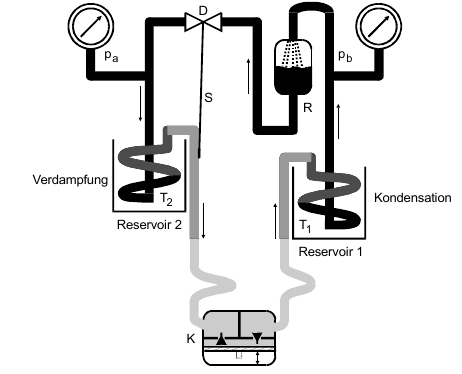
\includegraphics{WärmepunpeSchematisch1.png}
    \caption{Schematische Darstellung einer Wärmepumpe}
    \label{fig:schema}
\end{figure}
Das Gas durchläuft also einen Kreislauf, der angetrieben wird durch den Kompressor. Hier wird das Gas komprimiert, sodass es sich stark erwärmt während der Druck 
ebenfalls steigt. Im Reservoir 1 geht das Gas dann in den flüssigen Zustand über und überträgt eine Kondensationswärme, die das Medium im Reservoir aufheizt. 
In einem Reiniger wird das flüssige Medium von Gasblasen getrennt, da diese das Drosslerventil unbenutzbar machen würden. Das Ventil dient dazu, durch Aufbau
eines Strömungswiderstandes einen Druckunterschied aufzubauen. Im Reservoir 2 verdampft das Medium und entzieht dem Reservoir damit eine Wärmemenge. Also ist 2
das kältere Reservoir, aus dem Wärmeenergie an das heißere Reservoir 1 übertragen wird.
Die Steuervorrichtung S beeinflusst das Ventil durch die Temperaturdifferenz zwischen Eingang und Ausgang von Reservoir 2: ist diese unter einem Schwellenwert,
wird weniger Medium vom Ventil durchgelassen. 
Die mechanische Arbeit wird dabei am Kompressor zugeführt.

\subsection{Güteziffer}
Bezeichnen wir die Wärmemenge, die dem heißeren Reservoir zugefügt wird mit $Q_{1}$ und die zugehörige Temperatur mit $T_{1}$, die dem kälteren Reservoir entnommene 
Wärmemenge mit $Q_{2}$ und die zugehörige Temperatur $T_{2}$ sowie die aufgewandte Arbeit als $A$.
Die Güteziffer $\nu$ bezeichnet dann das Verhältnis von der übertragenen Wärmemenge zur aufgewandten Arbeit, es gilt also:
\begin{equation}
\nu = \frac{Q_{1}}{A}
\end{equation}
Je geringer also die nötige Arbeit oder je größer die aufgenommene Energie ist, desto größer ist die Güteziffer. 
Setzen wir zum einen voraus, dass die Wärmeübertragung ein reversibler Prozess ist, der prinzipiell genau so in die andere Richtung ablaufen könnte, sodass sämtliche
aufgewandte Energie wieder vollständig zurückgewonnen werden kann, und zum anderen, dass die Temperatur in den jeweiligen Reservoiren annährend gleich bleibt, gilt
nach dem zweiten Hauptsatz der Thermodynamik:
\begin{equation}
\nu_\text{ideal} = \frac{Q_1}{A} = \frac{T_1}{T_{1}-T_{2}}
\end{equation}
Offensichtlich ist das technisch nicht umsetzbar, da in der Praxis stets ein Teil verloren geht durch Wärmeleitung der verewendeten Rohre und Ähnlichem. Realistisch
ist also folgende Gleichung:
\begin{equation}
\nu_\text{real} < \frac{T_1}{T_{1}-T_{2}}
\end{equation}
Um die reale Güteziffer genau zu bestimmen, muss der Differenzenquotient $\frac{\increment T_1}{\increment t}$ aus der gemessenen Temperaturkurve betrachtet werden.
Daraus folgt für die Wärmemenge pro Zeiteinheit, mit der Wärmekapazität des Wassers $m_1 c_w$ und der Wärmekapazität der Kupferschlange und des 
Eimers $m_k c_k$:
\begin{equation}
\frac{\increment Q_1}{\increment t} = \left( m_1 c_w + m_k c_k \right) \frac{\increment T_1}{\increment t}
\end{equation}
Für die Güteziffer gilt dann widerum:
\begin{align}
\nu_\text{real} = \frac{\increment Q_1}{\increment t N}\\
= \left( m_1 c_w + m_k c_k \right) \frac{\increment T_1}{\increment t N}
\end{align}
Dabei werden also die Verluste berücksichtigt, die technisch nicht zu vermeiden sind; es wird ein irreversibles Szenario betrachtet.
Anhand dieser Gleichungen erkennt man leicht, dass die Güteziffer insbesodere von der Temperaturdifferenz abhängig ist. Je kleiner die Diffrenz ist, desto
weniger Arbeit muss verrichtet werden, um das heißere Reservoir aufzuheizen.
Die Güteziffer zeigt vor allem, welchen Vorteil die Wärmepumpe gegenüber den vorher genannten direkten Verfahren hat: bei direkten Verfahren ist die Wärmemenge
kleiner oder gleich der verrichteten Arbeit, während für die Wärmepumpe gilt:
\begin{equation}
Q_1 = A \frac{T_1}{T_1 - T_2}
\end{equation}

\subsection{Massendurchsatz}
Als Massendurchsatz bezeichnet man den Massenstrom durch ein Volumen pro Zeit. In einer Wärmepumpe wird ein Transportmedium verdampft, wodurch pro Zeit- und
Masseneinheit eine bestimmte Verdampfungswärme L verbraucht wird. \\
Ähnlich wie bei der Güteziffer wird ein Differenzenquotient betrachtet, diesmal der für den Verlauf der Temperatur von Reservoir 2:
\begin{equation}
\frac{\increment Q_2}{\increment t} = \left( m_2 c_w + m_k c_k \right) \frac{\increment T_2}{\increment t}
\end{equation}
Für die Verdampfungswärme L gilt:
\begin{equation}
\label{eq:neun}
\frac{\increment Q_2}{\increment t} = L \frac{\increment m}{\increment t}
\end{equation}
Setzen wir das gleich, um den Massendurchsatz zu berechnen:
\begin{align}
L \frac{\increment m}{\increment t} = \left( m_2 c_w + m_k c_k \right) \frac{\increment T_2}{\increment t}\\
\leftrightarrow \frac{\increment m}{\increment t} = \left( m_2 c_w + m_k c_k \right) \frac{\increment T_2}{\increment t} \frac{1}{L}
\end{align}
Es muss also L bekannt sein.

\subsection{mechanische Kompressorleistung}
Die mechanische Kompressorleistung gibt der Kompressor ab, wenn er das Gas von einem Volumen $V_a$ auf ein geringeres Volumen $V_b$ komprimiert. Da die
Leistung $N = \frac{\increment A}{\increment t}$ ist, und für die Arbeit, die ein Kompressor verrichtet, allgemein gilt
\begin{equation}
A_m = - \int_{V_a}^{V_b} p dV
\end{equation}
Für adiabatische Kompressionen gilt in der Thermodynamik die Poisson-Gleichung 
\begin{equation}
p_a V_a^{\kappa} = p_b V_b^{\kappa} = pV^{\kappa}
\end{equation}
Wobei $\kappa$ das Verhältnis der molaren Wärmen $C_p$ und $C_v$ bezeichnet, es ist immer größer als eins. Setzt man dies in die obige Formel ein, erhält man:
\begin{equation}
A_m = -p_a V_a^{\kappa} \int_{V_a}^{V_b} V^{- \kappa} dV = \frac{1}{\kappa - 1} p_a V_a^{\kappa} \left( V_b^{- \kappa + 1} - V_a^{- \kappa + 1} \right) =
    \frac{1}{\kappa - 1} \left( p_b \sqrt{\frac{p_a}{p_b}} - p_a \right) V_a
\end{equation}
Für die mechanische Kompressorleistung folgt also:
\begin{equation}
N_\text{mech} = \frac{\increment A_m}{\increment t} = \frac{1}{\kappa - 1} \left( p_b \sqrt{\frac{p_a}{p_b}} - p_a \right) \increment V_a
    =  \frac{1}{\kappa - 1} \left( p_b \sqrt{\frac{p_a}{p_b}} - p_a \right) \frac{1}{\rho} \frac{\increment m}{\increment t}
\end{equation}
Dabei ist $\rho$ die Dichte des Transportmediums beim Druck $p_a$. Mithilfe der idealen Gasgleichung \\ lässt sich der Wert errechnen.
Verwendet man Funktionen für die Messwerte für Temperaturen und Zeit, lassen sich die Differenzenquotienten durch Differentialquotienten ersetzen.